\documentclass[../thesis.tex]{subfiles}

\begin{document}
\section{Overall Description}
\subsection{Product Perspective}
% Đối với các cửa tiệm tạm hóa, qui trình theo dõi và ghi chép các sổ sách và giấy tờ sẽ tốn nhiều thời thời và công sức. Một chiếc tablet hay điện thoại có thể thay thế quyển sổ ghi truyền thống giúp tiết kiệm chi phí, thời gian và công sức của người chủ cửa tiệm. Song song đó  tránh mất mát các thông tin quan trọng, và cập nhật thông tin hoạt động được nhanhchóng và một cách chính xác nhất.
% Trên thực tế, các mô hình kinh bán nhỏ lẻ như vậy sẽ có một người đứng ra quản lý, thông thường sẽ là chủ tiệm.   Vậy nên để thuận tiện cho việc quản lý được hiệu quả nhất có thể và tạo sự đơn giản trong thiết kế giao diện nên hệ thống chỉ có môt tác nhân duy nhất Người Dùng
% Người dùng có chức năng xác minh người dùng bao gồm đăng nhập, đăng xuất và đăng xuất. Sau khi xác thực, người dùng  có thể truy cập các chức năng phục vụ việc quản lý, cụ thể:
% Quản lý kho hàng: Quản lý hàng tồn kho, Quản lý sản phẩm và Quản lý danh mục
% Quản lý bán hàng: Tạo hóa đơn, Quản lý hóa đơn, In hóa đơn, Quản lý thu chi.
% Quản lý thông tin cửa hàng: Quản lý nhà cung cấp, Quản lý khách hàng và thông tin cửa hàng.

Information systems in management are being widely applied in all fields of society in general and in business industries in particular. Mobile devices today such as smartphones and tablets are not only purely personal entertainment devices, but also provide strong support in handling tasks.

For small retail stores, the process of tracking and recording books and documents can be time-consuming and labor-intensive. A tablet or phone can replace traditional notebooks, saving costs, time and effort for the store owner. At the same time, it avoids the loss of important information and updates operational information quickly and accurately.


In practice, such small retail models will have a manager, usually the store owner. Therefore, to facilitate the most effective management possible and to simplify the interface design, the system should have only one agent: the User.

The user has user authentication functions including login, sign up and logout. After authentication, the user can access management functions, specifically:
\begin{itemize}
    \item[]\textbf{ Inventory management: }Manage inventory, manage products and manage categories.
    \item[]\textbf{ Sales management: }Create invoice, manage invoices, print invoices and manage revenue and expenditure.
    \item[]\textbf{ Store information management:} Manage suppliers, manage customers and store information.

\end{itemize}
% Các chức năng chính của hệ thống
\subsection{Product Functions}

\begin{enumerate}
    \item \textbf{User Authentication:} This feature allows the user to securely access the system by providing login and sign up logout functionality.
    \item \textbf{Inventory Management:} This feature enables the user to effectively manage the store's inventory by providing the following sub-features:
          \begin{itemize}
              \item \textbf{Inventory Tracking:} Allows the user to track the quantity and status of items in stock.
              \item \textbf{Product Management:} Enables the user to add, edit and delete products in the system.
              \item \textbf{Category Management:} Allows the user to organize products into categories for easier management.
          \end{itemize}
    \item \textbf{Sales Management:} This feature facilitates the sales process by providing the following sub-features:
          \begin{itemize}
              \item \textbf{Invoice Creation:} Allows the user to Create invoice for sales transactions.
              \item \textbf{Invoice Management:} Enables the user to view, edit and delete invoices.
              \item \textbf{Invoice Printing:} Allows the user to print invoices for record-keeping and customer reference.
              \item \textbf{Revenue and Expenditure Management:} Enables the user to track and manage the store's revenue and expenditure.
          \end{itemize}
    \item \textbf{Store Information Management:} This feature enables the user to manage information related to the store by providing the following sub-features:
          \begin{itemize} \item \textbf{Supplier Management:} Allows the user to add, edit and delete supplier information.
              \item \textbf{Customer Management:} Enables the user to add, edit and delete customer information.

          \end{itemize}

\end{enumerate}
\begin{figure}[H]
    \centering
    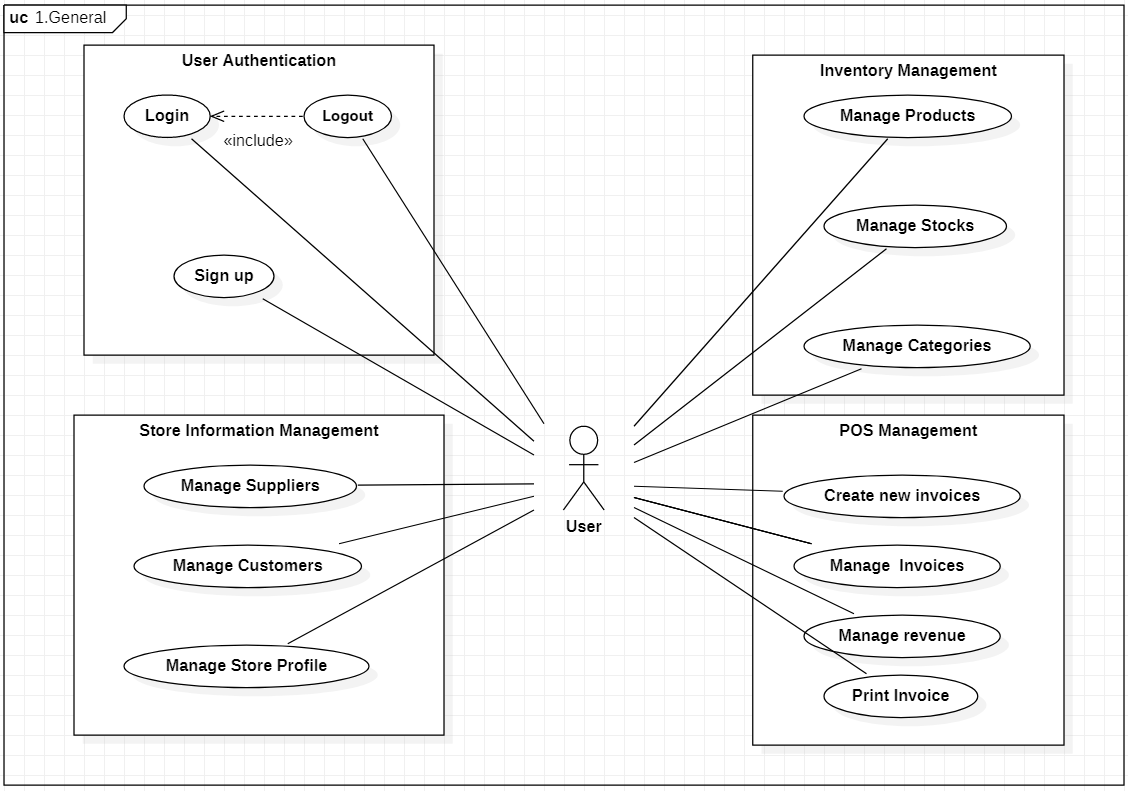
\includegraphics[width=1\textwidth]{images/UCD_General.png}
    \caption{General Usecase}
    \label{fig:UCD_General}
\end{figure}
%  Các yêu cầu phi chức năng
\subsection{User Classes and Characteristics}
% User Class: Store Owner/Manager
% Authentication: The user has the ability to authenticate themselves through login and sign up logout functions on the mobile application.
% Inventory Management: Once authenticated, the user can access the inventory management function on the mobile application which allows them to manage inventory, products, and categories. This information is stored and retrieved from a remote database.
% Sales Management: The user can also access the sales management function on the mobile application which allows them to create and manage invoices, print invoices, and manage revenue and expenditure. This information is also stored and retrieved from a remote database.
% Store Information Management: The user can access the store information management function on the mobile application which allows them to manage suppliers, customers, and store information. This information is also stored and retrieved from a remote database.
% Môi trường vận hành
\begin{itemize}
    \item[-] \textbf{User Class:} Store Owner/Manager
    \item[-] \textbf{Authentication:} The user has the ability to authenticate themselves through login, sign up and logout functions on the mobile application. This ensures that only authorized users have access to the management functions.
    \item[-] \textbf{Inventory Management:} Once authenticated, the user can access the inventory management function on the mobile application which allows them to manage inventory, products, and categories.
    \item[-] \textbf{Sales Management:} The user can also access the sales management function on the mobile application which allows them to create and manage invoices, print invoices, and manage revenue and expenditure.
    \item[-] \textbf{Store Information Management:} The user can access the store information management function on the mobile application which allows them to manage suppliers, customers, and store information.
    \item []All information is stored and retrieved from a remote database, allowing for real-time updates and accurate tracking of inventory levels, sales transactions, and store information.
\end{itemize}
\subsection{Operating Environment}
% các ràng buộc về thực thi và thiết kế
\section{Requirements Specification}
% Các giả định phụ thuộc
\subsection{External Interface Requirements}
\begin{itemize}
    \item[-]\textbf{User Interfaces:} The system should have a user-friendly interface on the mobile application for the store owner/manager to access and use the various management functions. The interface should be designed to be easy to navigate and intuitive to use.
    \item[-]\textbf{Hardware Interfaces:} The system should be compatible with common mobile devices such as smartphones and tablets. It should also be able to connect to a remote database server through a network connection.
    \item[-]\textbf{Software Interfaces:} The system should be able to interface with the remote database server to store and retrieve information. It should also be able to interface with other software systems such as accounting or inventory management software if necessary.
    \item[-]\textbf{Communication Interfaces:} The system should be able to communicate with the remote database server through a secure network connection. It should also be able to communicate with other devices or systems if necessary.

\end{itemize}

\subsection{Functional Requirement}
\subsubsection{Login}
\begin{figure}[H]
    \centering
    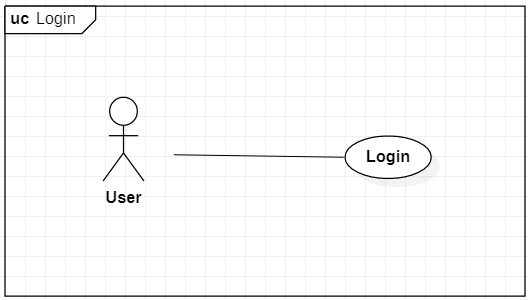
\includegraphics[width=0.75\textwidth]{images/UCD_Login.png}
    \caption{UC01a.Login}
    \label{fig:UCD-login}
\end{figure}
\begin{center}
    \begin{table}[H]
        % {|p{0.3\textwidth}|p{0.7\textwidth}|}
        \resizebox{0.95\textwidth}{!}{%
            \normalsize
            \begin{tabular}[htbp]{|p{0.25\textwidth}|p{0.75\textwidth}|}
                \hline
                \textbf{Use case}                & User Authentication: Log in                                                                                                    \\ \hline
                \textbf{ID }                     & UC01a                                                                                                                          \\ \hline
                \textbf{Main actor }             & User                                                                                                                           \\ \hline
                \textbf{Priority   }             & High                                                                                                                           \\ \hline
                \textbf{Brief description }      & Allows the user to securely access the system by providing login functionality.                                                \\ \hline
                \textbf{Trigger            }     & The user opens the application and selects the login option.                                                                   \\ \hline
                \textbf{Type             }       & Primary                                                                                                                        \\ \hline
                \textbf{Relationship        }    &                                                                                                                                \\ \hline
                \textbf{Normal flows         }   & \begin{enumerate}
                                                       \item The user opens the application.
                                                       \item  User enters email and password
                                                       \item The system verifies the credentials.
                                                       \item  The user is granted access to the system.
                                                       \item The user can access additional functions such as inventory management, sales management and store information management.
                                                       \item End login event
                                                   \end{enumerate} \\ \hline
                \textbf{Subflows              }  &                                                                                                                                \\ \hline
                \textbf{Exceptional flow       } & \begin{enumerate}
                                                       \item The user enters incorrect login credentials.
                                                       \item The system displays an error message and prompts the user to try again.
                                                   \end{enumerate}                                                   \\ \hline
            \end{tabular}%
        }
        \caption{User Authentication: Log in}
        \label{tab:table-usecase-user-login}


    \end{table}
\end{center}

\subsubsection{Sign up}
\begin{figure}[H]
    \centering
    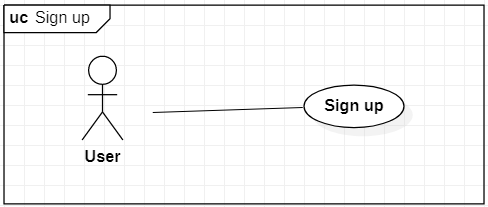
\includegraphics[width=0.75\textwidth]{images/UCD_Signup.png}
    \caption{UC01b.Sign up}
    \label{fig:UCD-sign-up}
\end{figure}
\begin{center}
    \begin{table}[H]
        % {|p{0.3\textwidth}|p{0.7\textwidth}|}
        \resizebox{0.95\textwidth}{!}{%
            \normalsize
            \begin{tabular}[htbp]{|p{0.25\textwidth}|p{0.75\textwidth}|}
                \hline
                \textbf{Use case}                & User Authentication: Sign up                                                                                                   \\ \hline
                \textbf{ID }                     & UC01b                                                                                                                          \\ \hline
                \textbf{Main actor }             & User                                                                                                                           \\ \hline
                \textbf{Priority   }             & High                                                                                                                           \\ \hline
                \textbf{Brief description }      & Allows the user to create an account in the system.                                                                            \\ \hline
                \textbf{Trigger            }     & The user opens the application to create an account.                                                                           \\ \hline
                \textbf{Type             }       & Primary                                                                                                                        \\ \hline
                \textbf{Relationship        }    &                                                                                                                                \\ \hline
                \textbf{Normal flows         }   & \begin{enumerate}
                                                       \item The user opens the application.
                                                       \item  User enters required information: Name,  Address and User credentials User's Email/Phone and Password.
                                                       \item The system verifies the credentials.
                                                       \item  System verifies information and creates a new account for the user.
                                                       \item  The user is granted access to the system.
                                                       \item The user can access additional functions such as inventory management, sales management and store information management.
                                                       \item End sign up event
                                                   \end{enumerate} \\ \hline
                \textbf{Subflows              }  &                                                                                                                                \\ \hline
                \textbf{Exceptional flow       } & \begin{enumerate}
                                                       \item System error while accessing sign up feature.
                                                       \item The system displays an error message and prompts the user to try again.
                                                   \end{enumerate}                                                   \\ \hline
            \end{tabular}%
        }
        \caption{User Authentication: Sign up}
        \label{tab:table-usecase-signup}


    \end{table}
\end{center}
\subsubsection{Log out}
\begin{figure}[H]
    \centering
    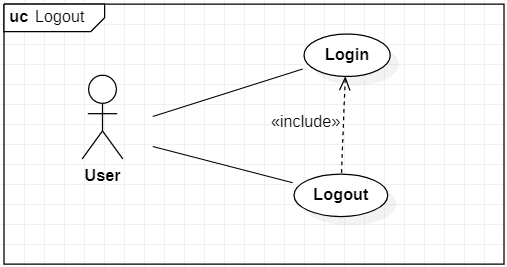
\includegraphics[width=0.75\textwidth]{images/UCD_Logout.png}
    \caption{UC01c.Log out}
    \label{fig:UCD-logout}
\end{figure}
\begin{center}
    \begin{table}[H]
        % {|p{0.3\textwidth}|p{0.7\textwidth}|}
        \resizebox{0.95\textwidth}{!}{%
            \normalsize
            \begin{tabular}[htbp]{|p{0.25\textwidth}|p{0.75\textwidth}|}
                \hline
                \textbf{Use case}                & User Authentication: Logout                                                  \\ \hline
                \textbf{ID }                     & UC01c                                                                        \\ \hline
                \textbf{Main actor }             & User                                                                         \\ \hline
                \textbf{Priority   }             & High                                                                         \\ \hline
                \textbf{Brief description }      & Allows the user to securely log out of the system.                           \\ \hline
                \textbf{Trigger            }     & User wants to log out of the system.                                         \\ \hline
                \textbf{Type             }       & Primary                                                                      \\ \hline
                \textbf{Relationship        }    &                                                                              \\ \hline
                \textbf{Normal flows         }   & \begin{enumerate}
                                                       \item User logs into the system (UC01a)
                                                       \item  User navigates to logout feature.
                                                       \item System logs user out of the system.
                                                       \item  User is no longer able to access the system until they log in again.
                                                       \item End log out event
                                                   \end{enumerate}   \\ \hline
                \textbf{Subflows              }  &                                                                              \\ \hline
                \textbf{Exceptional flow       } & \begin{enumerate}
                                                       \item The system displays an error message and prompts the user to try again.
                                                   \end{enumerate} \\ \hline
            \end{tabular}%
        }
        \caption{User Authentication: Log out}
        \label{tab:table-usecase-logout}


    \end{table}
\end{center}

\subsubsection{Manage Stock}
\begin{figure}[H]
    \centering
    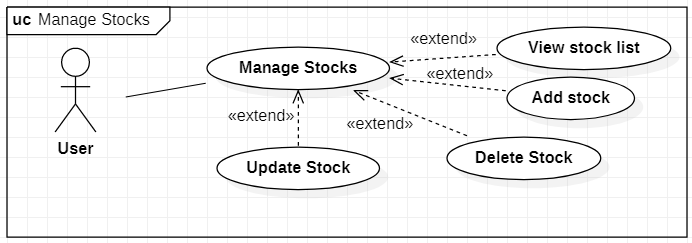
\includegraphics[width=0.75\textwidth]{images/UCD_ManageStock.png}
    \caption{UC02a.Manage Stock}
    \label{fig:UCD-manage-stock}
\end{figure}
\begin{center}
    \begin{table}[H]
        % {|p{0.3\textwidth}|p{0.7\textwidth}|}
        \resizebox{0.95\textwidth}{!}{%
            \normalsize
            \begin{tabular}[htbp]{|p{0.25\textwidth}|p{0.75\textwidth}|}
                \hline
                \textbf{Use case}                & Inventory Management: Manage Stock                                  \\ \hline
                \textbf{ID }                     & UC02a                                                               \\ \hline
                \textbf{Main actor }             & User                                                                \\ \hline
                \textbf{Priority   }             & High                                                                \\ \hline
                \textbf{Brief description }      & Allows the user to track the quantity and status of items in stock. \\ \hline
                \textbf{Trigger            }     & User wants to track inventory.                                      \\ \hline
                \textbf{Type             }       & Primary                                                             \\ \hline
                \textbf{Relationship        }    & Include UC01a                                                       \\ \hline
                \textbf{Normal flows         }   & \begin{enumerate}
                                                       \item User logs into the system (UC01a).
                                                       \item  User navigates to inventory tracking feature.
                                                       \item System displays inventory tracking interface.
                                                       \item  User views and updates inventory information as needed.
                                                       \item End of use case.
                                                   \end{enumerate}       \\ \hline
                \textbf{Subflows              }  &                                                                     \\ \hline
                \textbf{Exceptional flow       } & \begin{enumerate}
                                                       \item System error while accessing inventory tracking feature.
                                                   \end{enumerate}       \\ \hline
            \end{tabular}%
        }
        \caption{Inventory Management: Manage Stock}
        \label{tab:table-usecase-inventory-tracking}


    \end{table}
\end{center}
\subsubsection{Manage Products	}
\begin{figure}[H]
    \centering
    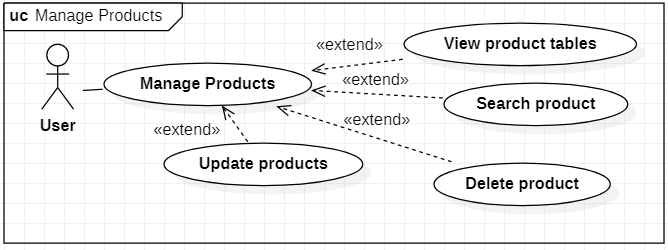
\includegraphics[width=0.75\textwidth]{images/UCD_ManageProducts.png}
    \caption{UC02b.Manage Products}
    \label{fig:UCD-manage-products}
\end{figure}
\begin{center}
    \begin{table}[H]
        % {|p{0.3\textwidth}|p{0.7\textwidth}|}
        \resizebox{0.95\textwidth}{!}{%
            \normalsize
            \begin{tabular}[htbp]{|p{0.25\textwidth}|p{0.75\textwidth}|}
                \hline
                \textbf{Use case}                & Inventory Management: Manage Products                           \\ \hline
                \textbf{ID }                     & UC02b                                                           \\ \hline
                \textbf{Main actor }             & User                                                            \\ \hline
                \textbf{Priority   }             & High                                                            \\ \hline
                \textbf{Brief description }      & Allows the user to add, edit and delete products in the system. \\ \hline
                \textbf{Trigger            }     & User wants to track inventory.                                  \\ \hline
                \textbf{Type             }       & Primary                                                         \\ \hline
                \textbf{Relationship        }    & Include  UC01a                                                  \\ \hline
                \textbf{Normal flows         }   & \begin{enumerate}
                                                       \item User logs into the system (UC01a).
                                                       \item  User navigates to product management feature.
                                                       \item System displays product management interface.
                                                       \item  User adds, edits or deletes products as needed.
                                                       \item End of use case.
                                                   \end{enumerate}           \\ \hline
                \textbf{Subflows              }  &                                                                 \\ \hline
                \textbf{Exceptional flow       } & \begin{enumerate}
                                                       \item System error while accessing product management feature.
                                                   \end{enumerate}   \\ \hline
            \end{tabular}%
        }
        \caption{Inventory Management: Manage Products}
        \label{tab:table-usecase-manage-products}


    \end{table}
\end{center}
\subsubsection{Manage Categories}
\begin{figure}[H]
    \centering
    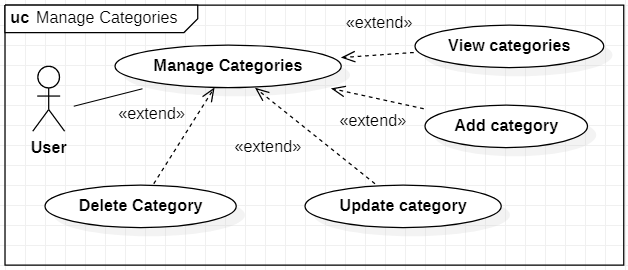
\includegraphics[width=0.8\textwidth]{images/UCD_ManageCategories.png}
    \caption{UC02c.Manage Categories}
    \label{fig:UCD_manage-categories}
\end{figure}
\begin{center}
    \begin{table}[H]
        % {|p{0.3\textwidth}|p{0.7\textwidth}|}
        \resizebox{0.95\textwidth}{!}{%
            \normalsize
            \begin{tabular}[htbp]{|p{0.25\textwidth}|p{0.75\textwidth}|}
                \hline
                \textbf{Use case}                & Inventory Management: Manage Categories                         \\ \hline
                \textbf{ID }                     & UC02c                                                           \\ \hline
                \textbf{Main actor }             & User                                                            \\ \hline
                \textbf{Priority   }             & High                                                            \\ \hline
                \textbf{Brief description }      & Allows the user to add, edit and delete categories in the system. \\ \hline
                \textbf{Trigger            }     & User wants to track inventory.                                  \\ \hline
                \textbf{Type             }       & Primary                                                         \\ \hline
                \textbf{Relationship        }    & Include UC01a                                                   \\ \hline
                \textbf{Normal flows         }   & \begin{enumerate}
                                                       \item User logs into the system (UC01a).
                                                       \item  User navigates to product category management.
                                                       \item System displays category management interface.
                                                       \item  User adds, edits or deletes categories as needed.
                                                       \item End of use case.
                                                   \end{enumerate}         \\ \hline
                \textbf{Subflows              }  &                                                                 \\ \hline
                \textbf{Exceptional flow       } & \begin{enumerate}
                                                       \item System error while accessing category management feature.
                                                   \end{enumerate}  \\ \hline
            \end{tabular}%
        }
        \caption{Inventory Management: Manage categories}
        \label{tab:table-usecase-manage-categories}


    \end{table}
\end{center}
\subsubsection{Create invoice}
\begin{figure}[H]
    \centering
    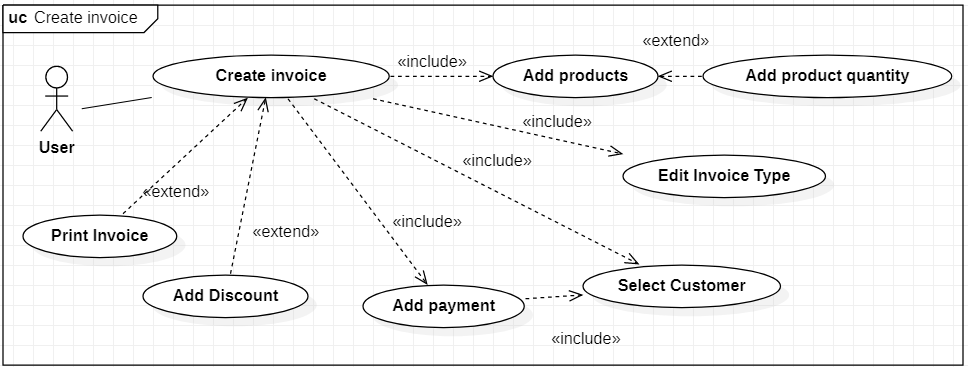
\includegraphics[width=1\textwidth]{images/UCD_CreateInvoice.png}
    \caption{UC03a.Create Invoice}
    \label{fig:UCD-create-invoice}
\end{figure}
\begin{center}
    \begin{table}[H]
        % {|p{0.3\textwidth}|p{0.7\textwidth}|}
        \resizebox{0.95\textwidth}{!}{%
            \normalsize
            \begin{tabular}[htbp]{|p{0.25\textwidth}|p{0.75\textwidth}|}
                \hline
                \textbf{Use case}                & Sales Management: Create invoice                                                                                                                                                                                                                                                                                                                  \\ \hline
                \textbf{ID }                     & UC03a                                                                                                                                                                                                                                                                                                                                              \\ \hline
                \textbf{Main actor }             & User                                                                                                                                                                                                                                                                                                                                               \\ \hline
                \textbf{Priority   }             & High                                                                                                                                                                                                                                                                                                                                               \\ \hline
                \textbf{Brief description }      & Allows the user to Create invoice for sales transactions.                                                                                                                                                                                                                                                                                         \\ \hline
                \textbf{Trigger            }     & User wants to create an invoice.                                                                                                                                                                                                                                                                                                                   \\ \hline
                \textbf{Type             }       & Primary                                                                                                                                                                                                                                                                                                                                            \\ \hline
                \textbf{Relationship        }    & Include UC01a                                                                                                                                                                                                                                                                                                                                      \\ \hline
                \textbf{Normal flows         }   & \begin{enumerate}
                                                       \item User logs into the system (UC01a).
                                                       \item User navigates to invoice creation feature.
                                                       \item System displays invoice creation interface.
                                                       \item User input required products and product quantity.Then input customer if invoice is order and option discount.
                                                       \item End of use case.
                                                   \end{enumerate}\\ \hline
                \textbf{Subflows              }  & \begin{enumerate}
                                                       \item User adds products to the invoice and update the quantity of products as needed.
                                                       \item Select invoice type.
                                                       \item  User enters customer information.
                                                       \item User applies discounts or promotions.
                                                       \item Add full payment if retail or add customer payment if customer invoices
                                                   \end{enumerate}\\ \hline
                \textbf{Exceptional flow       } & \begin{enumerate}
                                                       \item System error while accessing invoice creation feature.
                                                   \end{enumerate} \\ \hline
            \end{tabular}%
        }
        \caption{Sales Management: Create Invoice}
        \label{tab:table-usecase-create-invoice}


    \end{table}
\end{center}
\subsubsection{Manage Invoices}
\begin{figure}[H]
    \centering
    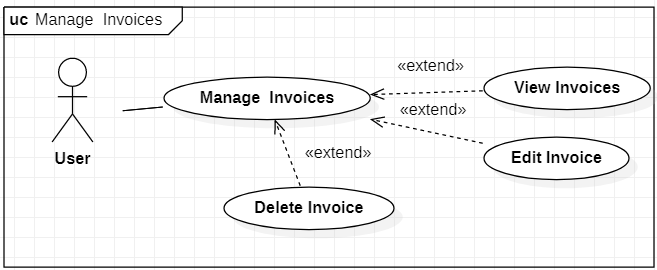
\includegraphics[width=0.8\textwidth]{images/UCD_ManageInvoices.png}
    \caption{UC03b.Manage Invoices}
    \label{fig:UCD-manage-invoices}
\end{figure}
\begin{center}
    \begin{table}[H]
        % {|p{0.3\textwidth}|p{0.7\textwidth}|}
        \resizebox{0.95\textwidth}{!}{%
            \normalsize
            \begin{tabular}[htbp]{|p{0.25\textwidth}|p{0.75\textwidth}|}
                \hline
                \textbf{Use case}                & Sales Management: Manage invoices                                                  \\ \hline
                \textbf{ID }                     & UC03b                                                                              \\ \hline
                \textbf{Main actor }             & User                                                                               \\ \hline
                \textbf{Priority   }             & High                                                                               \\ \hline
                \textbf{Brief description }      & Enables the user to view, edit and delete invoices.	User wants to manage invoices. \\ \hline
                \textbf{Trigger            }     & User wants to track inventory.                                                     \\ \hline
                \textbf{Type             }       & Primary                                                                            \\ \hline
                \textbf{Relationship        }    & Include UC01a, UC03a                                                                      \\ \hline
                \textbf{Normal flows         }   & \begin{enumerate}
                                                       \item User logs into the system (UC01a).
                                                       \item  User navigates to invoice management feature.
                                                       \item System displays invoice management interface.
                                                       \item  User views, edits or deletes invoices as needed.
                                                       \item End of use case.
                                                   \end{enumerate}                             \\ \hline
                \textbf{Subflows              }  &                                                                                    \\ \hline
                \textbf{Exceptional flow       } & \begin{enumerate}
                                                       \item System error while accessing invoice management feature.
                                                   \end{enumerate}                     \\ \hline
            \end{tabular}%
        }
        \caption{Sales Management: Manage Invoices}
        \label{tab:table-usecase-manage-invoices}
    \end{table}
\end{center}
\subsubsection{Manage Revenue and Expenditure}
\begin{figure}[H]
    \centering
    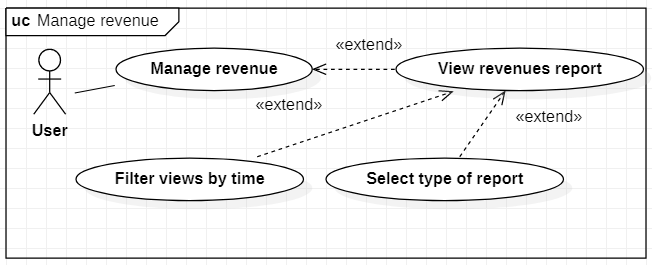
\includegraphics[width=0.8\textwidth]{images/UCD_ManageRevenue.png}
    \caption{UC03c.Manage Revenue}
    \label{fig:UCD-manage-revenue}
\end{figure}
\begin{center}
    \begin{table}[H]
        % {|p{0.3\textwidth}|p{0.7\textwidth}|}
        \resizebox{0.95\textwidth}{!}{%
            \normalsize
            \begin{tabular}[htbp]{|p{0.25\textwidth}|p{0.75\textwidth}|}
                \hline
                \textbf{Use case}                & Sales Management: Manage Revenue and Expenditure                                  \\ \hline
                \textbf{ID }                     & UC03c                                                                             \\ \hline
                \textbf{Main actor }             & User                                                                              \\ \hline
                \textbf{Priority   }             & High                                                                              \\ \hline
                \textbf{Brief description }      & Enables the user to track and manage the store’s revenue and expenditure.         \\ \hline
                \textbf{Trigger            }     & User wants to manage revenue and expenditure.                                     \\ \hline
                \textbf{Type             }       & Primary                                                                           \\ \hline
                \textbf{Relationship        }    & Include UC01a                                                                     \\ \hline
                \textbf{Normal flows         }   & \begin{enumerate}
                                                       \item User logs into the system (UC01a).
                                                       \item  User navigates to revenue and expenditure management feature.
                                                       \item System displays revenue and expenditure management interface.
                                                       \item  User views and updates views revenue and expenditure information as needed.
                                                       \item End of use case.
                                                   \end{enumerate} \\ \hline
                \textbf{Subflows              }  &                                                                                   \\ \hline
                \textbf{Exceptional flow       } & \begin{enumerate}
                                                       \item System error while accessing revenue and expenditure management feature.
                                                   \end{enumerate}      \\ \hline
            \end{tabular}%
        }
        \caption{Sales Management: Manage Revenue and Expenditure}
        \label{tab:table-usecase-manage-revenue-expenditure}
    \end{table}
\end{center}
\subsubsection{Print Invoices}
\begin{figure}[H]
    \centering
    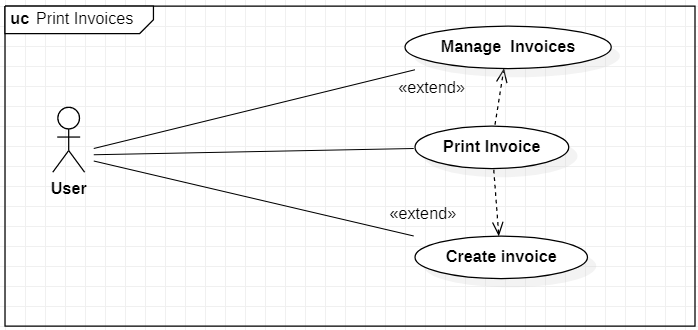
\includegraphics[width=0.75\textwidth]{images/UCD_PrintInvoice.png}
    \caption{UC03d.Print Invoice}
    \label{fig:UCD-print-invoice}
\end{figure}
\begin{center}
    \begin{table}[H]
        % {|p{0.3\textwidth}|p{0.7\textwidth}|}
        \resizebox{0.95\textwidth}{!}{%
            \normalsize
            \begin{tabular}[htbp]{|p{0.25\textwidth}|p{0.75\textwidth}|}
                \hline
                \textbf{Use case}                & Sales Management: Print Invoices                                  \\ \hline
                \textbf{ID }                     & UC03d                                                                             \\ \hline
                \textbf{Main actor }             & User                                                                              \\ \hline
                \textbf{Priority   }             & High                                                                              \\ \hline
                \textbf{Brief description }      & Allows the user to print invoices for record-keeping and customer reference.         \\ \hline
                \textbf{Trigger            }     & User wants to print an invoice.                                     \\ \hline
                \textbf{Type             }       & Primary                                                                           \\ \hline
                \textbf{Relationship        }    & Include UC01a, Extend UC03a ,  UC03b                                                               \\ \hline
                \textbf{Normal flows         }   & \begin{enumerate}
                                                       \item User logs into the system (UC01a).
                                                       \item  User navigates to invoice printing feature from UC03a ,  UC03b.
                                                       \item System displays invoice printing interface.
                                                       \item User selects printer and modify printing formats as needed.
                                                       \item  System prints the selected invoice.
                                                       \item End of use case.
                                                   \end{enumerate} \\ \hline
                \textbf{Subflows              }  &                                                                                   \\ \hline
                \textbf{Exceptional flow       } & \begin{enumerate}
                                                       \item System error while accessing printer or printing feature.
                                                   \end{enumerate}      \\ \hline
            \end{tabular}%
        }
        \caption{Sales Management: Print Invoices}
        \label{tab:table-usecase-print-invoices}
    \end{table}
\end{center}
\subsubsection{Manage Suppliers}
\begin{figure}[H]
    \centering
    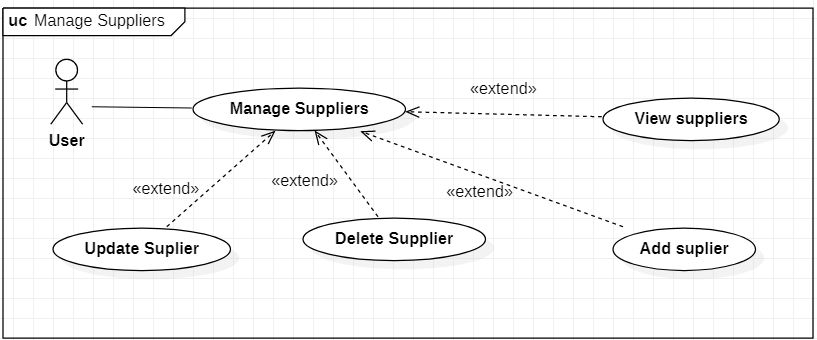
\includegraphics[width=0.75\textwidth]{images/UCD_ManageSuppliers.png}
    \caption{UC04a.Manage Suppliers}
    \label{fig:UCD-manage-suppliers}
\end{figure}
\begin{center}
    \begin{table}[H]
        % {|p{0.3\textwidth}|p{0.7\textwidth}|}
        \resizebox{0.95\textwidth}{!}{%
            \normalsize
            \begin{tabular}[htbp]{|p{0.25\textwidth}|p{0.75\textwidth}|}
                \hline
                \textbf{Use case}                & Store Information Management: Manage Suppliers                                    \\ \hline
                \textbf{ID }                     & UC04a                                                                             \\ \hline
                \textbf{Main actor }             & User                                                                              \\ \hline
                \textbf{Priority   }             & High                                                                              \\ \hline
                \textbf{Brief description }      & Allows the user to add, edit and delete supplier information.         \\ \hline
                \textbf{Trigger            }     & User wants to manage supplier information.                                    \\ \hline
                \textbf{Type             }       & Primary                                                                           \\ \hline
                \textbf{Relationship        }    & Include UC01a                                                              \\ \hline
                \textbf{Normal flows         }   & \begin{enumerate}
                                                       \item User logs into the system (UC01a).
                                                       \item  User navigates to supplier management feature.
                                                       \item System displays supplier management interface.
                                                       \item User adds, edits or deletes supplier information as needed.
                                                       \item End of use case.
                                                   \end{enumerate} \\ \hline
                \textbf{Subflows              }  &                                                                                   \\ \hline
                \textbf{Exceptional flow       } & \begin{enumerate}
                                                       \item System error while accessing supplier management feature
                                                   \end{enumerate}      \\ \hline
            \end{tabular}%
        }
        \caption{Store Information Management: Manage Suppliers}
        \label{tab:table-usecase-manage-suppliers}
    \end{table}
\end{center}
\subsubsection{Manage Customers}
\begin{figure}[H]
    \centering
    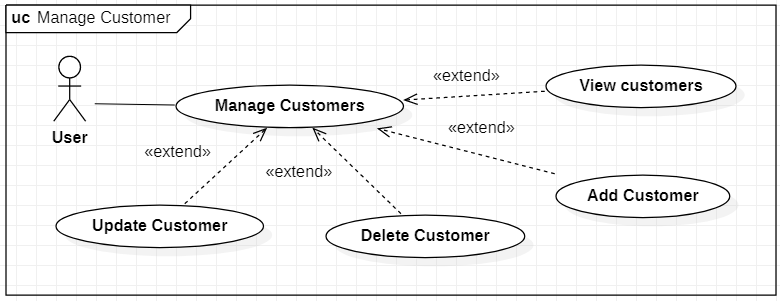
\includegraphics[width=0.75\textwidth]{images/UCD_ManageCustomers.png}
    \caption{UC04b.Manage Customers}
    \label{fig:UCD-manage-customers}
\end{figure}
\begin{center}
    \begin{table}[H]
        % {|p{0.3\textwidth}|p{0.7\textwidth}|}
        \resizebox{0.95\textwidth}{!}{%
            \normalsize
            \begin{tabular}[htbp]{|p{0.25\textwidth}|p{0.75\textwidth}|}
                \hline
                \textbf{Use case}                & Store Information Management: Manage Customers                                 \\ \hline
                \textbf{ID }                     & UC04b                                                                             \\ \hline
                \textbf{Main actor }             & User                                                                              \\ \hline
                \textbf{Priority   }             & High                                                                              \\ \hline
                \textbf{Brief description }      & Allows the user to add, edit and delete customer information.         \\ \hline
                \textbf{Trigger            }     & User wants to manage customer information.                                    \\ \hline
                \textbf{Type             }       & Primary                                                                           \\ \hline
                \textbf{Relationship        }    & Include UC01a                                                              \\ \hline
                \textbf{Normal flows         }   & \begin{enumerate}
                                                       \item User logs into the system (UC01a).
                                                       \item  User navigates to customer management feature.
                                                       \item System displays customer management interface.
                                                       \item User adds, edits or deletes customer information as needed.
                                                       \item End of use case.
                                                   \end{enumerate} \\ \hline
                \textbf{Subflows              }  &                                                                                   \\ \hline
                \textbf{Exceptional flow       } & \begin{enumerate}
                                                       \item System error while accessing customer management feature
                                                   \end{enumerate}      \\ \hline
            \end{tabular}%
        }
        \caption{Store Information Management: Manage Customers}
        \label{tab:table-usecase-manage-customers}
    \end{table}
\end{center}
\subsubsection{Manage Store}
\begin{figure}[H]
    \centering
    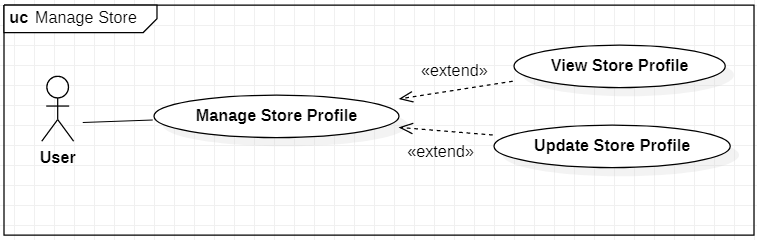
\includegraphics[width=0.75\textwidth]{images/UCD_ManageStoreInfo.png}
    \caption{UC04c.Manage Store}
    \label{fig:UCD-manage-store-info}
\end{figure}
\begin{center}
    \begin{table}[H]
        % {|p{0.3\textwidth}|p{0.7\textwidth}|}
        \resizebox{0.95\textwidth}{!}{%
            \normalsize
            \begin{tabular}[htbp]{|p{0.25\textwidth}|p{0.75\textwidth}|}
                \hline
                \textbf{Use case}                & Sales Management: Print Invoices                                  \\ \hline
                \textbf{ID }                     & UC04c                                                                             \\ \hline
                \textbf{Main actor }             & User                                                                              \\ \hline
                \textbf{Priority   }             & High                                                                              \\ \hline
                \textbf{Brief description }      & Allows the user to edit basic store information such as store name, address and contact.         \\ \hline
                \textbf{Trigger            }     & User wants to edit basic store information.                                  \\ \hline
                \textbf{Type             }       & Primary                                                                           \\ \hline
                \textbf{Relationship        }    & Include UC01a                                                              \\ \hline
                \textbf{Normal flows         }   & \begin{enumerate}
                                                       \item User logs into the system (UC01a).
                                                       \item  User navigates to store information feature.
                                                       \item System displays store information interface.
                                                       \item User edits basic store information such as store name, address and contact.
                                                       \item End of use case.
                                                   \end{enumerate} \\ \hline
                \textbf{Subflows              }  &                                                                                   \\ \hline
                \textbf{Exceptional flow       } & \begin{enumerate}
                                                       \item System error while accessing store information feature.
                                                   \end{enumerate}      \\ \hline
            \end{tabular}%
        }
        \caption{Store Information Management: Manage Store Information}
        \label{tab:table-usecase-manage-store-info}
    \end{table}
\end{center}
\subsection{Nonfunctional Requirements}
% MỤC TIÊU CẦN ĐẠT ĐƯỢC
% CƠ SỞ LÝ THUYẾT
\end{document}